\documentclass[a4paper,11pt,oneside]{book}
\usepackage{amsmath} %Never write a paper without using amsmath for its many new commands
\usepackage{amssymb} %Some extra symbols
\usepackage{makeidx} %If you want to generate an index, automatically
\usepackage{graphicx} %If you want to include postscript graphicsfor example.
\usepackage{hyperref}
\usepackage{color}
\usepackage{tocloft}		% fancy TOC
\usepackage{fncychap}	% fancy Chapter title

\makeindex
  
% -----------------------------------------------------------------------------------------
% hyperlinks
% -----------------------------------------------------------------------------------------
\hypersetup{
    colorlinks=false,       % false: boxed links; true: colored links
    %linkbordercolor={204 204 204},
    linkcolor=red,          % color of internal links
    colorlinks,%
    citecolor=black,%
    filecolor=black,%
    linkcolor=black,%
    urlcolor=black
}

% -----------------------------------------------------------------------------------------
% support for chars like <>, used e.g. in #include <
% -----------------------------------------------------------------------------------------
\usepackage[T1]{fontenc} % for handeling chars like < >  etc

% -----------------------------------------------------------------------------------------
% page headers and footer style
% -----------------------------------------------------------------------------------------
\usepackage{fancyhdr}
\pagestyle{fancy}

% -----------------------------------------------------------------------------------------
% titlepage
% -----------------------------------------------------------------------------------------

% -----------------------------------------------------------------------------------------
% page margin formatting, less marging than default
% -----------------------------------------------------------------------------------------
\usepackage[lmargin=2.5cm,rmargin=2.5cm,tmargin=2.5cm,bmargin=2.5cm]{geometry}

% -----------------------------------------------------------------------------------------
% paragraph formatting
% -----------------------------------------------------------------------------------------
\setlength{\parindent}{0pt}
\setlength{\parskip}{1ex plus 0.5ex minus 0.2ex}

% -----------------------------------------------------------------------------------------
% source code formatting settings
% -----------------------------------------------------------------------------------------
\usepackage{listings}
\definecolor{sourcecode}{RGB}{255,255,255}
\lstset{ %
	basicstyle=\footnotesize,
	frame=single,
	captionpos=b,
	breaklines=true,
	backgroundcolor=\color{sourcecode}
}

% -----------------------------------------------------------------------------------------
% libfunction 
% -----------------------------------------------------------------------------------------
\definecolor{libfunctionbg}{RGB}{192,192,192}
\definecolor{sublibfunctionbg}{RGB}{255,255,255}
\newcommand{\libfunction}[1] {\vspace{10 mm} \noindent \colorbox{libfunctionbg}{\parbox{\textwidth}{\Large\textbf{#1}}} }
\newcommand{\sublibfunction}[1] {\vspace{10 mm} \par\noindent\colorbox{sublibfunctionbg}{\makebox[\textwidth][l]{\large\itshape\textbf{#1}}} }


\newcommand{\HRule}{\rule{\linewidth}{0.5mm}}


% #######################################################

\title{The Quant Finance Code Library: C++ Random}
%\author{M.A. (Thijs) van den Berg}
\date{\today}

\begin{document}
%\maketitle
\begin{titlepage}

\begin{center}


\begin{picture}(0,0)
        \put(-40,0){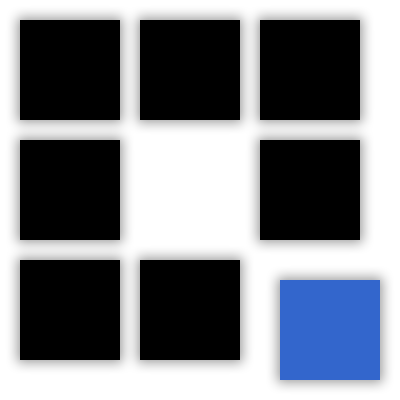
\includegraphics[scale=0.10]{qlogo.png}}
        \put(-90,26){
            \parbox[t]{90mm}{
            \begin{flushright}
            \textsf{\Large Quant Finance Code Library}
            \end{flushright}
            }
        }
\end{picture}\\[3.14cm]


% Title
\rule{\textwidth}{1pt}\par \vspace{0.5\baselineskip}
{\fontfamily{phv}\fontsize{128pt}{128pt}\selectfont Random}\\[0.5cm]
{\fontfamily{phv}\fontsize{60pt}{60pt}\selectfont C++}\\[0.5cm]
{\fontfamily{phv}\fontsize{60pt}{60pt}\selectfont Library}\\[0.5cm]
\rule{\textwidth}{1pt}\par \vspace{0.5\baselineskip}

% Author and supervisor
\begin{minipage}[t]{0.4\textwidth}
\begin{flushleft} \large
\emph{Authors:}\\
Thijs van den \textsc{Berg}\\

\end{flushleft}
\end{minipage}
\begin{minipage}[t]{0.4\textwidth}
\begin{flushright} \large
\emph{Contributors:} \\
Thijs \textsc{van den Berg}\\
James \textsc{Hirschorn}
\end{flushright}
\end{minipage}

\vfill

% Bottom of the page
{\large \today}

\end{center}

\end{titlepage}
\tableofcontents

\mainmatter
% ----------------------------------------------------------------------------------------------
\newpage
\chapter{Overview}
The QFCL Random C++ library covers routines used for generating samples from various probability distribution.


\section{\index{Engines}Engines}
Engines generate random numbers with certain properties. The C++ standard library, the BOOST libraries provide various random
number engines. The engines in QFCL adhere to the same interfaces and are thus interoperable with C++ and BOOST random related routines. 

The Engines provided in QFCL have two major benefits:
\begin{itemize}
\item They are thread safe.
\item These engines can generate parallel independent random streams.
\end{itemize}
Both features are requires for efficient parallel random number generation and in parallel Monte Carlo engines.

\subsection{Interface}
Engines provide the following interface
\begin{itemize}
\item operator() for generating random numbers.
\item max() that returns the higher random number that can be generated.
\item min() that returns the lowest random number that can be generated.
\end{itemize}

\section{\index{Distribution}Distribution}
todo


\section{Generating variates}
todo

\begin{lstlisting}[ language=C++,
                    caption=Creating Vanilla call price sampler,
                    emph={gbm_npv_vanilla_call},
                    emphstyle=\bf\color{blue}]
    
    typedef qfcl::random::cpp_rand ENG;
    typedef qfcl::random::gbm_npv_vanilla_call DIST;
    typedef qfcl::random::variate_generator< ENG, DIST > RNG;
    
    double S0 = 100;
    double vol = 0.25;
    double yield = 0.05;
    double r = 0.05; 
    double strike = 110;
    double t = 1.5;
    
    DIST call( S0, vol, yield, r, strike, t );
    ENG eng;
    RNG rng(eng,call);
    
    for (int i=0;i<1000; ++i) 
    	std::cout << rng() << "\n";
\end{lstlisting}

% ----------------------------------------------------------------------------------------------
\newpage
\chapter{Engines}


\section{\index{MersenneTwister}Mersenne Twister}
todo

\section{\index{Philox}Counter based Philox}
todo
% ----------------------------------------------------------------------------------------------
\newpage
\chapter{Distributions}

\section{\index{Uniform}Uniform Distributions}
% ------------------------------------------------------------------------------------------------
%
% ------------------------------------------------------------------------------------------------
\sublibfunction{Description}
The distribution uniform\_0ex\_1ex\_distribution and it's variants are used to generate samples
from uniform distributions. The ex and in keyword indicate exclusion of inclusion of 0 and/or 1 in the generated 
samples.

\begin{tabular}{ | l | l | }
  \hline
  distribution & range \\
  \hline                        
  uniform\_0ex\_1ex & $(0,1)$ \\
  uniform\_0in\_1ex & $[0,1)$ \\
  uniform\_0ex\_1in & $(0,1]$ \\
  uniform\_0in\_1in & $[0,1]$ \\
  \hline  
\end{tabular}

% ------------------------------------------------------------------------------------------------
%
% ------------------------------------------------------------------------------------------------
\subsection{uniform\_0ex\_1ex}
\sublibfunction{Synopsis}
\begin{lstlisting}[language=C++]
// Include files
#include <qfcl/random/distribution/uniform_0ex_1ex.hpp>

// Types
template<class RealType = double>  class uniform_0ex_1ex_distribution;

// convenience typedef
typedef uniform_0ex_1ex_distribution <double> uniform_0ex_1ex;
\end{lstlisting}


% ------------------------------------------------------------------------------------------------
%
% ------------------------------------------------------------------------------------------------
\subsection{uniform\_0ex\_1in}
\sublibfunction{Synopsis}
\begin{lstlisting}[language=C++]
// Include files
#include <qfcl/random/distribution/uniform_0ex_1in.hpp>

// Types
template<class RealType = double>  class uniform_0ex_1in_distribution;

// convenience typedef
typedef uniform_0ex_1in_distribution <double> uniform_0ex_1in;
\end{lstlisting}


% ------------------------------------------------------------------------------------------------
%
% ------------------------------------------------------------------------------------------------
\subsection{uniform\_0in\_1ex}
\sublibfunction{Synopsis}
\begin{lstlisting}[language=C++]
// Include files
#include <qfcl/random/distribution/uniform_0in_1ex.hpp>

// Types
template<class RealType = double>  class uniform_0in_1ex_distribution;

// convenience typedef
typedef uniform_0in_1ex_distribution <double> uniform_0in_1ex;
\end{lstlisting}


% ------------------------------------------------------------------------------------------------
%
% ------------------------------------------------------------------------------------------------
\subsection{uniform\_0in\_1in}
\sublibfunction{Synopsis}
\begin{lstlisting}[language=C++]
// Include files
#include <qfcl/random/distribution/uniform_0in_1in.hpp>

// Types
template<class RealType = double>  class uniform_0in_1in_distribution;

// convenience typedef
typedef uniform_0in_1in_distribution <double> uniform_0in_1in;
\end{lstlisting}











% ------------------------------------------------------------------------------------------------
%
% ------------------------------------------------------------------------------------------------
\sublibfunction{Example}
\begin{lstlisting}[language=C++,caption=Sample C++ code: function interface,numbers=left]
#include <qfcl/random/engine/mersene_twister.hpp>
#include <qfcl/random/distribution/uniform_0in_1ex.hpp>
#include <qfcl/random/variate_generator.hpp>

int main()
{
    typedef qfcl::random::cpp_rand ENG;
    typedef qfcl::random::uniform_0in_1ex DIST;
    typedef qfcl::random::variate_generator< ENG, DIST > RNG;
    
    DIST u;
    ENG eng;
    RNG rng(eng,call);
    
    for (int i=0;i<1000; ++i) 
    	std::cout << rng() << "\n";
    return 0;
}
\end{lstlisting}



\section{\index{Normal}Normal Distributions}

% ------------------------------------------------------------------------------------------------
%
% ------------------------------------------------------------------------------------------------
\sublibfunction{Description}
The distributions normal\_xxx\_distribution are used to generate samples
from standard normal distributions. The xxx keyword indicate which method it uses to generate normal samples.

\begin{tabular}{ | l | l | }
  \hline                        
  distribution & method \\
  \hline                        
  normal\_box\_muller & Box Muller transform.\\
  normal\_box\_muller\_polar & Box Muller transform, polar variant.\\
  normal\_inversion & Using the inverse cumulative distribution function.\\
  \hline  
\end{tabular}


\subsection{normal\_box\_muller}
\sublibfunction{Synopsis}
\begin{lstlisting}[language=C++]
// Include files
#include <qfcl/random/distribution/normal_box_muller.hpp>

// Types
template<class RealType = double> class normal_box_muller_distribution;

// convenience typedef
typedef normal_box_muller_distribution<double> normal_box_muller;
\end{lstlisting}




\subsection{normal\_box\_muller\_polar}
\sublibfunction{Synopsis}
\begin{lstlisting}[language=C++]
// Include files
#include <qfcl/random/distribution/normal_box_muller_polar.hpp>

// Types
template<class RealType = double> class normal_box_muller_polar_distribution;

// convenience typedef
typedef normal_box_muller__polar_distribution<double> normal_box_muller_polar;
\end{lstlisting}


\subsection{normal\_inversion}
\sublibfunction{Synopsis}
\begin{lstlisting}[language=C++]
// Include files
#include <qfcl/random/distribution/normal_inversion.hpp>

// Types
template<class RealType = double> class normal_inversion_distribution;

// convenience typedef
typedef normal_inversion_distribution<double> normal_inversion;
\end{lstlisting}


% ------------------------------------------------------------------------------------------------
%
% ------------------------------------------------------------------------------------------------
\sublibfunction{Example}
\begin{lstlisting}[language=C++,caption=Sample C++ code: function interface,numbers=left]
#include <qfcl/random/engine/mersene_twister.hpp>
#include <qfcl/random/distribution/normal_inversion.hpp>
#include <qfcl/random/variate_generator.hpp>

int main()
{
    typedef qfcl::random::cpp_rand ENG;
    typedef qfcl::random::normal_inversion DIST;
    typedef qfcl::random::variate_generator< ENG, DIST > RNG;
    
    DIST n;
    ENG eng;
    RNG rng(eng,n);
    
    for (int i=0;i<1000; ++i) 
    	std::cout << rng() << "\n";
    return 0;
}
\end{lstlisting}



\section{\index{Gbm}Geometric Brownian Motion type Distributions}
\subsection{gbm\_at\_fixed\_time}
\sublibfunction{Description}
Sample from a fixed time distribution of geometric Brownian motion. 

todo

\subsection{gbm\_interval\_high}
todo
\subsection{gbm\_interval\_low}
todo
\subsection{gbm\_first\_hitting\_time}
todo

\subsection{gbm\_npv\_vanilla\_call}

% ------------------------------------------------------------------------------------------------
%
% ------------------------------------------------------------------------------------------------
\sublibfunction{Synopsis}
\begin{lstlisting}[language=C++]
// Include file
#include <qfcl/random/distribution/gbm_npv_vanilla_call.hpp>

// Types
template<class RealType = double> 
class gbm_vanilla_call_distribution;

// convenience typedef
typedef gbm_vanilla_call_distribution<double> gbm_vanilla_call;

\end{lstlisting}

% ------------------------------------------------------------------------------------------------
%
% ------------------------------------------------------------------------------------------------
\sublibfunction{Description}
The distribution gbm\_npv\_vanilla\_call\_distribution is used to generate samples
from a vanilla call option price. The underlying process is assumed to be a geometric Brownian Motion. 
The prices are npv-ed (net present valued).

% ------------------------------------------------------------------------------------------------
%
% ------------------------------------------------------------------------------------------------
\sublibfunction{Example}
\begin{lstlisting}[language=C++,caption=Sample C++ code: function interface,numbers=left]
#include <qfcl/random/engine/mersene_twister.hpp>
#include <qfcl/random/distribution/gbm_npv_vanilla_call.hpp>
#include <qfcl/random/variate_generator.hpp>

int main()
{
    typedef qfcl::random::cpp_rand ENG;
    typedef qfcl::random::gbm_npv_vanilla_call DIST;
    typedef qfcl::random::variate_generator< ENG, DIST > RNG;
    
    double S0 = 100;
    double vol = 0.25;
    double yield = 0.05;
    double r = 0.05; 
    double strike = 110;
    double t = 1.5;
    
    DIST call( S0, vol, yield, r, strike, t );
    ENG eng;
    RNG rng(eng,call);
    
    for (int i=0;i<1000; ++i) 
    	std::cout << rng() << "\n";
    return 0;
}
\end{lstlisting}



\subsection{gbm\_npv\_vanilla\_put}
todo

% ----------------------------------------------------------------------------------------------
\newpage
\chapter{Tutorial}
A tutorial that introduces the fundamental concepts required to use Qfcl.Random, 
and shows how to use Qfcl.Random to develop simple programs. 


\section{Headers and Namespaces}
All the code in this library is inside namespace qfcl::random. You can to bring distribution names into scope perhaps with a using namespace qfcl::random; declaration, but it's recommended that you use declarations like using qfcl::random::normal\_inversion; 


In order to generate samples from  a distribution some\_special\_distribution you will need to include either the
header <qfcl/random/distributions/some\_special.hpp> or the "include everything" 
header: <qfcl/random/distributions.hpp>.

\begin{lstlisting}[language=C++,caption=Including a "single distribution" header]
#include <qfcl/random/distributions/some_special.hpp>
\end{lstlisting}


\section{Distribution names and aliases}
All distribution are defined as templates with the real type  as argument and have names ending with "\_distribution".
E.g. the normal\_inversion\_distribution, is an distribution sampler that uses the inversion method to generate normal variates.

\begin{lstlisting}[language=C++,caption=]
// include file
#include <qfcl/random/distributions/normal_inversion.hpp>

// declaring a distribution
qfcl::random::normal_inversion_distribution<float> my_dist;
\end{lstlisting}

The real type of distribution defaults to double, and all distributions have a typedef omitting the \_distribution in the name for the double 
real type. The following declarations are all identical

\begin{lstlisting}[language=C++,caption=]
// verbose version
qfcl::random::normal_inversion_distribution<double> my_dist;

// using the default template type (double)
qfcl::random::normal_inversion_distribution<> my_dist;

// using the convenience typdef
qfcl::random::normal_inversion my_dist;
\end{lstlisting}


\backmatter
\bibliographystyle{amsalpha} %The style you want to use for references.
\bibliography{mr,refs} %The files containing all the articles and books you ever referenced.
\printindex %Make an index AUTOMATICALLY

\end{document} 